\section{Preliminaries}
\label{sec:HomographyPreliminaries}

In this section, we describe our established terminology. Even though there are standard conventions for naming certain aspects of our problem, we nevertheless had to invent few more terms to ease information delivery and improve clarity.

A~marker is an object with a known, easy-to-detect shape. This object is either naturally occurring or artificially placed on the planar surface of the scene we want to produce a bird's-eye view for, i.e., to remove perspective distortion. The marker contains keypoints, a set of distinct, independent, visual feature points, e.g., corners. The chosen keypoints visible in the perspectively deformed image are called the \mbox{warped keypoints}. The set of the \mbox{rectified keypoints} in the desired image (not subjected to perspective distortion) is produced from the warped keypoints using the homography projection. The \mbox{point correspondence} is a relationship between the warped and the \mbox{target keypoints} and it is used for homography estimation. Ideally, the rectified keypoints match the target keypoints. See Figure~\ref{fig:HomographyTerminology} for details.

\begin{figure}[t]
    \centering
    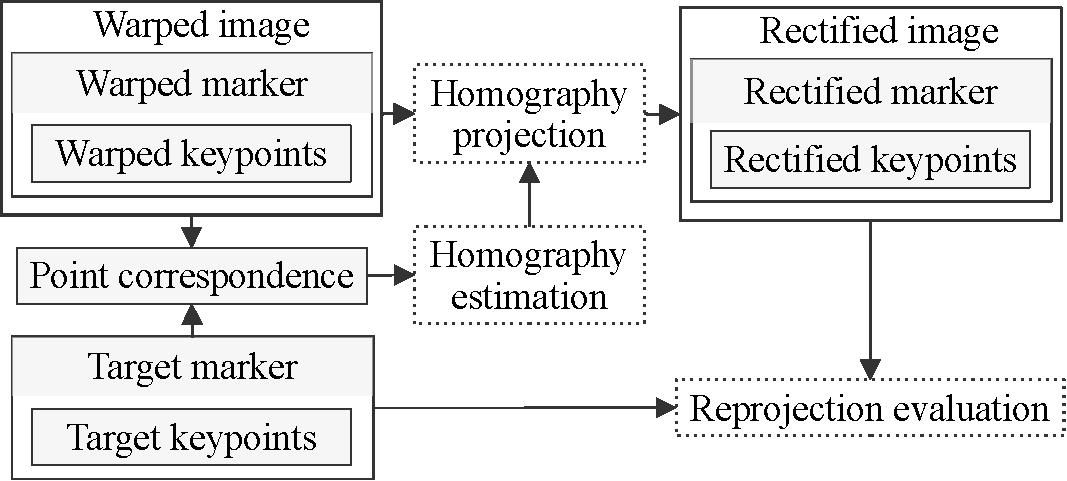
\includegraphics[width=0.6\linewidth]{figures/homography/terminology.pdf}
    \caption{Visualization of relationships in our established terminology. The diagram also shows the hierarchical dependence of individual terms. Dotted elements represent processes with arrows denoting their input and output.}
    \label{fig:HomographyTerminology}
\end{figure}

Without stating otherwise, a \mbox{\textbf{similarity transformation}} will denote a limited affine transformation with $4$ DoF consisting of translation, rotation and uniform scaling (equation \eqref{eq:SimilarityMatrices}). Let $\mset{K}_1$ and $\mset{K}_2$ be sets of feature keypoints belonging to objects $O_1$ and $O_2$. We say that objects $O_1$ and $O_2$ are \mbox{\textbf{similar}} if there exists a similarity transformation $\psi$, such that $\mset{K}_1 = \func{\psi}{\mset{K}_2}$ and $\mset{K}_2 = \func{\psi^{-1}}{\mset{K}_1}$. For example, $O_1$ and $O_2$ may be rectangles of different sizes but with an identical aspect ratio.

Let $m$ be the number of markers and $k$ be the number of keypoints of each marker. Each $i$-th marker is described by a $3 \times k$ matrix $\suprbrackets{\mtx{W}}{i}$ containing its warped keypoints as

\begin{equation}
    \suprbrackets{\mtx{W}}{i} =
    \begin{bmatrix}
        \subsuprbrackets{x}{1}{i} & \subsuprbrackets{x}{2}{i} & \dots & \subsuprbrackets{x}{k}{i} \\
        \subsuprbrackets{y}{1}{i} & \subsuprbrackets{y}{2}{i} & \dots & \subsuprbrackets{y}{k}{i} \\
        1                         & 1                         & \dots & 1
    \end{bmatrix},
    i = 1, \dots, m.
\end{equation}

\noindent The target keypoints are specified analogically by the $3 \times k$ matrix $\mtx{T}$. Only one specification is sufficient due to many-to-one correspondence. The ordering of keypoints needs to match the warped keypoints defined above. Thus,

\begin{equation}
    \mtx{T} =
    \begin{bmatrix}
        \tilde{x}_1 & \tilde{x}_2 & \dots & \tilde{x}_k \\
        \tilde{y}_1 & \tilde{y}_2 & \dots & \tilde{y}_k \\
        1           & 1           & \dots & 1
    \end{bmatrix},
\end{equation}

\noindent with the point correspondence being

\begin{equation}
    \subsuprbrackets{x}{j}{i} \simeq \tilde{x}_j, \subsuprbrackets{y}{j}{i} \simeq \tilde{y}_j, i = 1, \dots, m, j = 1, \dots, k.
\end{equation}

